%% abtex2-modelo-trabalho-academico.tex, v-1.9.7 laurocesar
%% Copyright 2012-2018 by abnTeX2 group at http://www.abntex.net.br/ 
%%
%% This work may be distributed and/or modified under the
%% conditions of the LaTeX Project Public License, either version 1.3
%% of this license or (at your option) any later version.
%% The latest version of this license is in
%%   http://www.latex-project.org/lppl.txt
%% and version 1.3 or later is part of all distributions of LaTeX
%% version 2005/12/01 or later.
%%
%% This work has the LPPL maintenance status `maintained'.
%% 
%% The Current Maintainer of this work is the abnTeX2 team, led
%% by Lauro César Araujo. Further information are available on 
%% http://www.abntex.net.br/
%%
%% This work consists of the files abntex2-modelo-trabalho-academico.tex,
%% abntex2-modelo-include-comandos and abntex2-modelo-references.bib
%%

% ------------------------------------------------------------------------
% ------------------------------------------------------------------------
% abnTeX2: Modelo de Trabalho Academico (tese de doutorado, dissertacao de
% mestrado e trabalhos monograficos em geral) em conformidade com 
% ABNT NBR 14724:2011: Informacao e documentacao - Trabalhos academicos -
% Apresentacao
% ------------------------------------------------------------------------
% ------------------------------------------------------------------------

\documentclass[
	% -- opções da classe memoir --
	12pt,				% tamanho da fonte
	openright,			% capítulos começam em pág ímpar (insere página vazia caso preciso)
	oneside,			% para impressão em recto e verso. Oposto a oneside
	a4paper,			% tamanho do papel. 
	% -- opções da classe abntex2 --
	chapter=TITLE,		% títulos de capítulos convertidos em letras maiúsculas
	section=TITLE,		% títulos de seções convertidos em letras maiúsculas
	%subsection=TITLE,	% títulos de subseções convertidos em letras maiúsculas
	%subsubsection=TITLE,% títulos de subsubseções convertidos em letras maiúsculas
	sumario=abnt-6027-2012,
	% -- opções do pacote babel --
	english,			% idioma adicional para hifenização
	french,				% idioma adicional para hifenização
	spanish,			% idioma adicional para hifenização
	brazil				% o último idioma é o principal do documento
	]{abntex2}

\renewcommand{\ABNTEXchapterfont}{\fontfamily{lmodern}}
\renewcommand{\ABNTEXchapterfont}{\fontseries{ub}}


\renewcommand{\ABNTEXsectionfont}{\normalfont}

% Altera as fontes no texto
\renewcommand{\chaptitlefont}{\normalfont\bfseries}
\setsecheadstyle{\normalfont\MakeUppercase}
\setsubsecheadstyle{\normalfont\bfseries}
\setsubsubsecheadstyle{\normalfont\bfseries\itshape}
\setsubsubsubsecheadstyle{\normalfont}


% ---
% Pacotes básicos 
% ---
\usepackage{lmodern}			% Usa a fonte Latin Modern			
\usepackage[T1]{fontenc}		% Selecao de codigos de fonte.
\usepackage[utf8]{inputenc}		% Codificacao do documento (conversão automática dos acentos)
\usepackage{lastpage}			% Usado pela Ficha catalográfica
\usepackage{indentfirst}		% Indenta o primeiro parágrafo de cada seção.
\usepackage{color}				% Controle das cores
\usepackage{graphicx}			% Inclusão de gráficos
%\usepackage{microtype} 		% para melhorias de justificação
\usepackage{amsmath}			% para o uso de ferramentas matemáticas
\usepackage{amssymb}
\usepackage{multirow}
\usepackage{subfloat}
\usepackage{pdfpages}
\usepackage{tikz}

\settocdepth{subsection}  

% ---

% ---
% Pacotes adicionais, usados apenas no âmbito do Modelo Canônico do abnteX2
% ---
\usepackage{lipsum}				% para geração de dummy text
% ---


% ---
% Pacotes para código
% ---

\usepackage{listings}
\usepackage{xcolor}

\definecolor{codegreen}{rgb}{0,0.6,0}
\definecolor{codegray}{rgb}{0.5,0.5,0.5}
\definecolor{codepurple}{rgb}{0.58,0,0.82}
\definecolor{backcolour}{rgb}{0.95,0.95,0.92}

\lstdefinestyle{mystyle}{
	backgroundcolor=\color{backcolour},
	commentstyle=\color{codegreen},
	keywordstyle=\color{magenta},
	numberstyle=\tiny\color{codegray},
	stringstyle=\color{codepurple},
	basicstyle=\ttfamily\tiny,
	breakatwhitespace=false,
	breaklines=true,
	captionpos=b,
	keepspaces=true,
	numbers=left,
	numbersep=4pt,
	showspaces=false,
	showstringspaces=false,
	showtabs=false,  
	tabsize=1
}

\lstset{style=mystyle}

% ---
% Pacotes de citações
% ---
\usepackage[brazilian, hyperpageref]{backref}	     % Paginas com as citações na bibl
\usepackage[bibjustif, num]{abntex2cite}	 % Citações padrão ABNT
\citebrackets()
\usepackage{lscape}


% --- 
% CONFIGURAÇÕES DE PACOTES
% --- 

% ---
% Configurações do pacote backref
% Usado sem a opção hyperpageref de backref
%\renewcommand{\backrefpagesname}{Citado na(s) página(s):~}
% Texto padrão antes do número das páginas
%\renewcommand{\backref}{}
% Define os textos da citação
%\renewcommand*{\backrefalt}[4]{
%	\ifcase #1 %
%		Nenhuma citação no texto.%
%	\or
%		Citado na página #2.%
%	\else
%		Citado #1 vezes nas páginas #2.%
%	\fi}%
% ---

% ---
% Informações de dados para CAPA e FOLHA DE ROSTO
% Quando o título está na forma TITULO: subtítulo todas as letras do título
% devem estar em maiúsculas e todas as do subtítulo em minúsculas

% ---
\titulo{MODELO CANÔNICO: exemplo de trabalho acadêmico com \abnTeX}
\autor{Nome do autor}
\local{Rio de Janeiro}
\data{2024}
\instituicao{%
	Programa de Pós-Graduação em Química
	\par
	Instituto de Química
	\par
	Universidade Federal do Rio de Janeiro - UFRJ}
\tipotrabalho{Tese (Doutorado)}
% O preambulo deve conter o tipo do trabalho, o objetivo, 
% o nome da instituição e a área de concentração 
\preambulo{Tese de Doutorado apresentada ao Programa de Pós-Graduação em Química (PGQu), do Instituto de Química da Universidade Federal do Rio de Janeiro, como parte dos requisitos necessários à obtenção do título de Doutor em Ciências.}
\orientador{Nome do Orientador}
\coorientador{Nome do Coorientador}
% ---


% ---
% Configurações de aparência do PDF final

% alterando o aspecto da cor azul
\definecolor{blue}{RGB}{41,5,195}

% informações do PDF
\makeatletter
\hypersetup{
	%pagebackref=true,
	pdftitle={\@title}, 
	pdfauthor={\@author},
	pdfsubject={\imprimirpreambulo},
	pdfcreator={LaTeX with abnTeX2},
	pdfkeywords={abnt}{latex}{abntex}{abntex2}{trabalho acadêmico}, 
	colorlinks=true,       		% false: boxed links; true: colored links
	linkcolor=black,          	% color of internal links
	citecolor=black,        		% color of links to bibliography
	filecolor=black,      		% color of file links
	urlcolor=black,
	bookmarksdepth=4,
	hidelinks
}
\makeatother
% --- 

% ---
% Posiciona figuras e tabelas no topo da página quando adicionadas sozinhas
% em um página em branco. Ver https://github.com/abntex/abntex2/issues/170
\makeatletter
\setlength{\@fptop}{5pt} % Set distance from top of page to first float
\makeatother
% ---

% ---
% Possibilita criação de Quadros e Lista de quadros.
% Ver https://github.com/abntex/abntex2/issues/176
%
\newcommand{\quadroname}{Quadro}
\newcommand{\listofquadrosname}{Lista de quadros}

\newfloat[chapter]{quadro}{loq}{\quadroname}
\newlistof{listofquadros}{loq}{\listofquadrosname}
\newlistentry{quadro}{loq}{0}

% configurações para atender às regras da ABNT
\setfloatadjustment{quadro}{\centering}
\counterwithout{quadro}{chapter}
\renewcommand{\cftquadroname}{\quadroname\space} 
\renewcommand*{\cftquadroaftersnum}{\hfill--\hfill}

\setfloatlocations{quadro}{hbtp} % Ver https://github.com/abntex/abntex2/issues/176
% ---

% --- 
% Espaçamentos entre linhas e parágrafos 
% --- 

% O tamanho do parágrafo é dado por:
\setlength{\parindent}{1.3cm}

% Controle do espaçamento entre um parágrafo e outro:
\setlength{\parskip}{0.2cm}  % tente também \onelineskip

% ---
% compila o indice
% ---
\makeindex
% ---

% ----
% Início do documento
% ----
\begin{document}

% Seleciona o idioma do documento (conforme pacotes do babel)
%\selectlanguage{english}
\selectlanguage{brazil}

% Retira espaço extra obsoleto entre as frases.
\frenchspacing 

% ----------------------------------------------------------
% ELEMENTOS PRÉ-TEXTUAIS
% ----------------------------------------------------------
% \pretextual

% ---
% Capa
% ---

% Impressão da Capa
\renewcommand{\imprimircapa}{
	\begin{capa}
		\center
		\begin{figure}
			\centering
			
\includegraphics[scale=0.65]{capitulos/figuras/ufrj-horizontal-cor-cmyk-completa-impressao}
			\label{minerva}
		\end{figure}
		
		
		\large INSTITUTO DE QUÍMICA \\ PROGRAMA DE PÓS-GRADUAÇÃO EM QUÍMICA \\NOME DO AUTOR
		
		\vfill
		\begin{center}
			\bfseries\LARGE\imprimirtitulo
		\end{center}
		\vfill
		
		Rio de Janeiro \\%\large\imprimirlocal %<<<<<<<<<<<mude
		2024 %\large\imprimirdata %<<<<<<<< mude
		
		\vspace*{1cm}
	\end{capa}
}
% ---

\imprimircapa
% ---

% ---
% Folha de rosto
% (o * indica que haverá a ficha bibliográfica)
% ---
\imprimirfolhaderosto*
% ---

% ---
% Inserir a ficha bibliografica
% ---

% Isto é um exemplo de Ficha Catalográfica, ou ``Dados internacionais de
% catalogação-na-publicação''. Você pode utilizar este modelo como referência:

%\begin{fichacatalografica}
%	\sffamily
%	\vspace*{\fill}					% Posição vertical
%	\begin{center}					% Minipage Centralizado
	%	\fbox{\begin{minipage}[c][8cm]{13.5cm}		% Largura
			%	\small
			%	\imprimirautor
			%Sobrenome, Nome do autor
			
			%	\hspace{0.5cm} \imprimirtitulo  / \imprimirautor. --
			%	\imprimirlocal, \imprimirdata-
			
			%	\hspace{0.5cm} \thelastpage p. : il. (algumas color.) ; 30 cm.\\
			
			%	\hspace{0.5cm} \imprimirorientadorRotulo~\imprimirorientador\\
			%	
			%	\hspace{0.5cm}
			%	\parbox[t]{\textwidth}{\imprimirtipotrabalho~--~\imprimirinstituicao,
				%	\imprimirdata.}\\
			%	
			%	\hspace{0.5cm}
			%		1. Palavra-chave1.
			%		2. Palavra-chave2.
			%		2. Palavra-chave3.
			%		I. Orientador.
			%		II. Universidade xxx.
			%		III. Faculdade de xxx.
			%		IV. Título 			
			%	\end{minipage}}
	%	\end{center}
%\end{fichacatalografica}
% ---


% A ficha pode ser gerada on-line em https://fichacatalografica.sibi.ufrj.br/
% Quando estiver com o documento, salve-o como PDF no diretório do seu projeto e 
% substitua todo o conteúdo de implementação deste arquivo pelo comando abaixo:
%
\begin{fichacatalografica}
	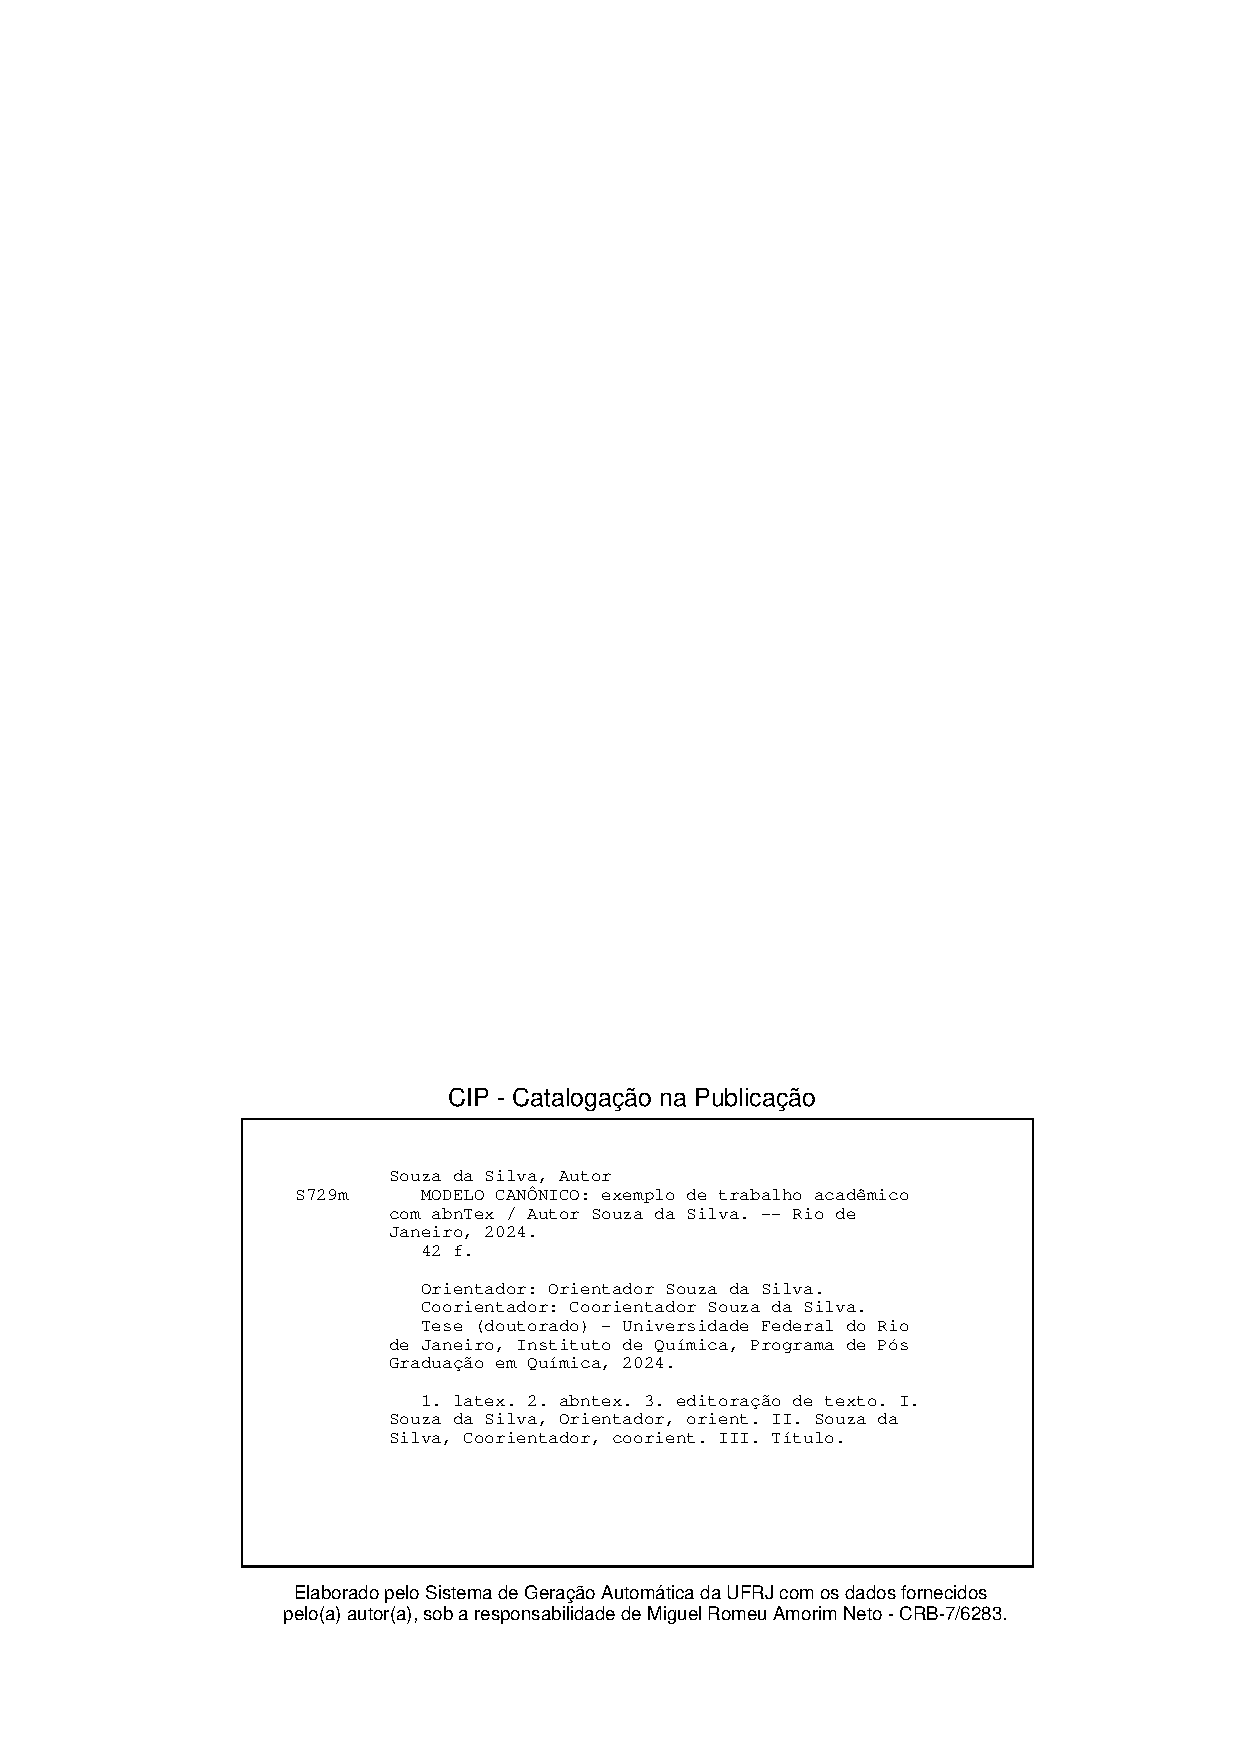
\includepdf{ficha_catalografica.pdf} 
\end{fichacatalografica}



% ---
% Inserir errata
% ---
\begin{errata}
Elemento opcional da \citeonline[4.2.1.2]{NBR14724:2011}. Exemplo:

\vspace{\onelineskip}

FERRIGNO, C. R. A. \textbf{Tratamento de neoplasias ósseas apendiculares com
reimplantação de enxerto ósseo autólogo autoclavado associado ao plasma
rico em plaquetas}: estudo crítico na cirurgia de preservação de membro em
cães. 2011. 128 f. Tese (Livre-Docência) - Faculdade de Medicina Veterinária e
Zootecnia, Universidade de São Paulo, São Paulo, 2011.

\begin{table}[htb]
\center
\footnotesize
\begin{tabular}{|p{1.4cm}|p{1cm}|p{3cm}|p{3cm}|}
  \hline
   \textbf{Folha} & \textbf{Linha}  & \textbf{Onde se lê}  & \textbf{Leia-se}  \\
    \hline
    1 & 10 & auto-conclavo & autoconclavo\\
   \hline
\end{tabular}
\end{table}

\end{errata}
% ---

% ---
% Inserir folha de aprovação
% ---

% Isto é um exemplo de Folha de aprovação, elemento obrigatório da NBR
% 14724/2011 (seção 4.2.1.3). Você pode utilizar este modelo até a aprovação
% do trabalho. Após isso, substitua todo o conteúdo deste arquivo por uma
% imagem da página assinada pela banca com o comando abaixo:
%
% \begin{folhadeaprovacao}
% \includepdf{folhadeaprovacao_final.pdf}
% \end{folhadeaprovacao}
%
\begin{folhadeaprovacao}

  \begin{center}
    {\ABNTEXchapterfont\large\imprimirautor}

    \vspace*{\fill}\vspace*{\fill}
    \begin{center}
      \ABNTEXchapterfont\bfseries\Large\imprimirtitulo
    \end{center}
    \vspace*{\fill}
    
    \hspace{.45\textwidth}
    \begin{minipage}{.5\textwidth}
        \imprimirpreambulo
    \end{minipage}%
    \vspace*{\fill}
   \end{center}
        
   Trabalho aprovado. \imprimirlocal, 24 de novembro de 2012:

   \assinatura{\textbf{\imprimirorientador} \\ Orientador} 
   \assinatura{\textbf{Prof. Dr. Interno 1 } \\ Afiliação - SIGLA}
   \assinatura{\textbf{Prof. Dr. Interno 2 } \\ Afiliação - SIGLA}
   \assinatura{\textbf{Prof. Dr. Externo 1 } \\ Afiliação - SIGLA}
   \assinatura{\textbf{Prof. Dr. Externo 2 } \\ Afiliação - SIGLA}

      
   \begin{center}
    \vspace*{0.5cm}
    {\large\imprimirlocal}
    \par
    {\large\imprimirdata}
    \vspace*{1cm}
  \end{center}
  
\end{folhadeaprovacao}
% ---

% ---
% Dedicatória
% ---
\begin{dedicatoria}
   \vspace*{\fill}
   \centering
   \noindent
   \textit{ Este trabalho é dedicado às crianças adultas que,\\
   quando pequenas, sonharam em se tornar cientistas.} \vspace*{\fill}
\end{dedicatoria}
% ---

% ---
% Agradecimentos
% ---
\begin{agradecimentos}
Os agradecimentos principais são direcionados à Gerald Weber, Miguel Frasson,
Leslie H. Watter, Bruno Parente Lima, Flávio de Vasconcellos Corrêa, Otavio Real
Salvador, Renato Machnievscz\footnote{Os nomes dos integrantes do primeiro
projeto abn\TeX\ foram extraídos de
\url{http://codigolivre.org.br/projects/abntex/}} e todos aqueles que
contribuíram para que a produção de trabalhos acadêmicos conforme
as normas ABNT com \LaTeX\ fosse possível.

Agradecimentos especiais são direcionados ao Centro de Pesquisa em Arquitetura
da Informação\footnote{\url{http://www.cpai.unb.br/}} da Universidade de
Brasília (CPAI), ao grupo de usuários
\emph{latex-br}\footnote{\url{http://groups.google.com/group/latex-br}} e aos
novos voluntários do grupo
\emph{\abnTeX}\footnote{\url{http://groups.google.com/group/abntex2} e
\url{http://www.abntex.net.br/}}~que contribuíram e que ainda
contribuirão para a evolução do \abnTeX.

\end{agradecimentos}
% ---

% ---
% Epígrafe
% ---
\begin{epigrafe}
	\vspace*{\fill}
	\begin{flushright}
		\textit{Tudo é infinto \\
			no mundo das ideias \\
			não há um fim p'r'o pensar. \\
			Ideias não têm limites \\}
	\end{flushright}
	
	\begin{flushright}
		\textit{Limites quem têm são pessoas \\
			(as mesmas que têm as ideias) \\
			são elas que lhes dão - às ideias - \\
			um limite, um fim \\
			que é delas - das pessoas -, só delas... só. \\}
	\end{flushright}
	
	\begin{flushright}
		\textit{Já as coisas da matéria \\
			elas sim, têm sempre um fim.\\
			São limitadas no tempo: \\
			um dia nascem, morrem um dia \\
			todas elas têm um fim. \\
			Também no espaço há limites \\
			que o vazio do entorno \\
			lhes contorna, lhes dá fim. \\}
	\end{flushright}
	
	\begin{flushright}
		(POETICES - Claudio Costa Neto )
	\end{flushright}
\end{epigrafe}
% ---

% ---
% RESUMOS
% ---

% resumo em português
\setlength{\absparsep}{18pt} % ajusta o espaçamento dos parágrafos do resumo
\begin{resumo}
 Segundo a \citeonline[3.1-3.2]{NBR6028:2003}, o resumo deve ressaltar o
 objetivo, o método, os resultados e as conclusões do documento. A ordem e a extensão
 destes itens dependem do tipo de resumo (informativo ou indicativo) e do
 tratamento que cada item recebe no documento original. O resumo deve ser
 precedido da referência do documento, com exceção do resumo inserido no
 próprio documento. (\ldots) As palavras-chave devem figurar logo abaixo do
 resumo, antecedidas da expressão Palavras-chave:, separadas entre si por
 ponto e finalizadas também por ponto.

 \textbf{Palavras-chave}: latex. abntex. editoração de texto.
\end{resumo}

% resumo em inglês
\begin{resumo}[Abstract]
 \begin{otherlanguage*}{english}
   This is the english abstract.

   \vspace{\onelineskip}
 
   \noindent 
   \textbf{Keywords}: latex. abntex. text editoration.
 \end{otherlanguage*}
\end{resumo}

% resumo em francês 
%\begin{resumo}[Résumé]
% \begin{otherlanguage*}{french}
%    Il s'agit d'un résumé en français.
 
%   \textbf{Mots-clés}: latex. abntex. publication de textes.
% \end{otherlanguage*}
%\end{resumo}

% resumo em espanhol
%\begin{resumo}[Resumen]
% \begin{otherlanguage*}{spanish}
%   Este es el resumen en español.
  
%   \textbf{Palabras clave}: latex. abntex. publicación de textos.
% \end{otherlanguage*}
%\end{resumo}
% ---

% ---
% inserir lista de ilustrações
% ---
\pdfbookmark[0]{\listfigurename}{lof}
\listoffigures*
\cleardoublepage
% ---

% ---
% inserir lista de quadros
% ---
\pdfbookmark[0]{\listofquadrosname}{loq}
\listofquadros*
\cleardoublepage
% ---

% ---
% inserir lista de tabelas
% ---
\pdfbookmark[0]{\listtablename}{lot}
\listoftables*
\cleardoublepage
% ---

% ---
% inserir lista de abreviaturas e siglas
% ---
\begin{siglas}
  \item[ABNT] Associação Brasileira de Normas Técnicas
  \item[abnTeX] ABsurdas Normas para TeX
\end{siglas}
% ---

% ---
% inserir lista de símbolos
% ---
\begin{simbolos}
  \item[$ \Gamma $] Letra grega Gama
  \item[$ \Lambda $] Lambda
  \item[$ \zeta $] Letra grega minúscula zeta
  \item[$ \in $] Pertence
\end{simbolos}
% ---

% ---
% inserir o sumario
% ---
\pdfbookmark[0]{\contentsname}{toc}
\tableofcontents*
\cleardoublepage
% ---



% ----------------------------------------------------------
% ELEMENTOS TEXTUAIS
% ----------------------------------------------------------
\textual

% ----------------------------------------------------------
% Faz com que o número das páginas somente apareça na primeira
% página da introdução. 
% ESSE VALOR DEVE SER ALTERADO MANUALMENTE!
% A CAPA NÂO É CONTADA
% ----------------------------------------------------------
\pagenumbering{arabic}
\setcounter{page}{17}

% ----------------------------------------------------------
% Capítulos escritos separadamente para melhor organização
% ----------------------------------------------------------

%% abtex2-modelo-include-comandos.tex, v-1.9.6 laurocesar
%% Copyright 2012-2016 by abnTeX2 group at http://www.abntex.net.br/ 
%%
%% This work may be distributed and/or modified under the
%% conditions of the LaTeX Project Public License, either version 1.3
%% of this license or (at your option) any later version.
%% The latest version of this license is in
%%   http://www.latex-project.org/lppl.txt
%% and version 1.3 or later is part of all distributions of LaTeX
%% version 2005/12/01 or later.
%%
%% This work has the LPPL maintenance status `maintained'.
%% 
%% The Current Maintainer of this work is the abnTeX2 team, led
%% by Lauro César Araujo. Further information are available on 
%% http://www.abntex.net.br/
%%
%% This work consists of the files abntex2-modelo-include-comandos.tex
%% and abntex2-modelo-img-marca.pdf
%%

% ---
% Este capítulo, utilizado por diferentes exemplos do abnTeX2, ilustra o uso de
% comandos do abnTeX2 e de LaTeX.
% ---

\chapter{Introdução}
\label{intro}
% ----------------------------------------------------------

Este documento e seu código-fonte são exemplos de referência de uso da classe \textsf{abntex2} e do pacote \textsf{abntex2cite}. O documento exemplifica a elaboração de trabalho acadêmico (tese, dissertação e outros do gênero) produzido conforme a ABNT NBR 14724:2011 \emph{Informação e documentação Trabalhos acadêmicos - Apresentação}.

A expressão ``Modelo Canônico'' é utilizada para indicar que \abnTeX\ não é modelo específico de nenhuma universidade ou instituição, mas que implementa tão somente os requisitos das normas da ABNT. Uma lista completa das normas observadas pelo \abnTeX\ é apresentada em \citeonline{abntex2classe}.

Sinta-se convidado a participar do projeto \abnTeX! Acesse o site do projeto em \url{http://www.abntex.net.br/}. Também fique livre para conhecer, estudar, alterar e redistribuir o trabalho do \abnTeX, desde que os arquivos modificados tenham seus nomes alterados e que os créditos sejam dados aos autores originais, nos termos da ``The \LaTeX\ Project Public License''\footnote{\url{http://www.latex-project.org/lppl.txt}}.

Encorajamos que sejam realizadas customizações específicas deste exemplo para universidades e outras instituições --- como capas, folha de aprovação, etc. Porém, recomendamos que ao invés de se alterar diretamente os arquivos do \abnTeX, distribua-se arquivos com as respectivas customizações. Isso permite que futuras versões do \abnTeX~não se tornem automaticamente incompatíveis com as customizações promovidas. Consulte \citeonline{abntex2-wiki-como-customizar} para mais informações.

Este documento deve ser utilizado como complemento dos manuais do \abnTeX\ \cite{abntex2classe,abntex2cite,abntex2cite-alf} e da classe \textsf{memoir} \cite{memoir}. 

Esperamos, sinceramente, que o \abnTeX\ aprimore a qualidade do trabalho que você produzirá, de modo que o principal esforço seja concentrado no principal: na contribuição científica.

Equipe \abnTeX 

Lauro César Araujo

	\section{Adição de figuras}
	
	A \autoref{intro:exemplo} apresenta um exemplo de figura criada em formato vetorial. Sempre prefira esse tipo de formato, pois ele apresenta maior qualidade tanto no formato digital quanto no formato impresso. Além disso, em geral ele gera arquivos muito mais leves, o que facilita a execução, armazenamento e transmissão da tese. Para gráficos muito complexos criados em Python, é recomendado utilizar a opção de rasterização para tornar a compilação do arquivo mais rápida. Mais detalhes podem ser encontrados em \url{https://matplotlib.org/stable/gallery/misc/rasterization_demo.html}.
		
	\begin{figure}[!h]
		\centering
		\caption{Exemplo de figura. As figuras devem ser criadas em formato PDF ou SVG sempre que possível. Quando não for possível, devem ser geradas em formato png com DPI superior a 600.}
		\label{intro:exemplo}
		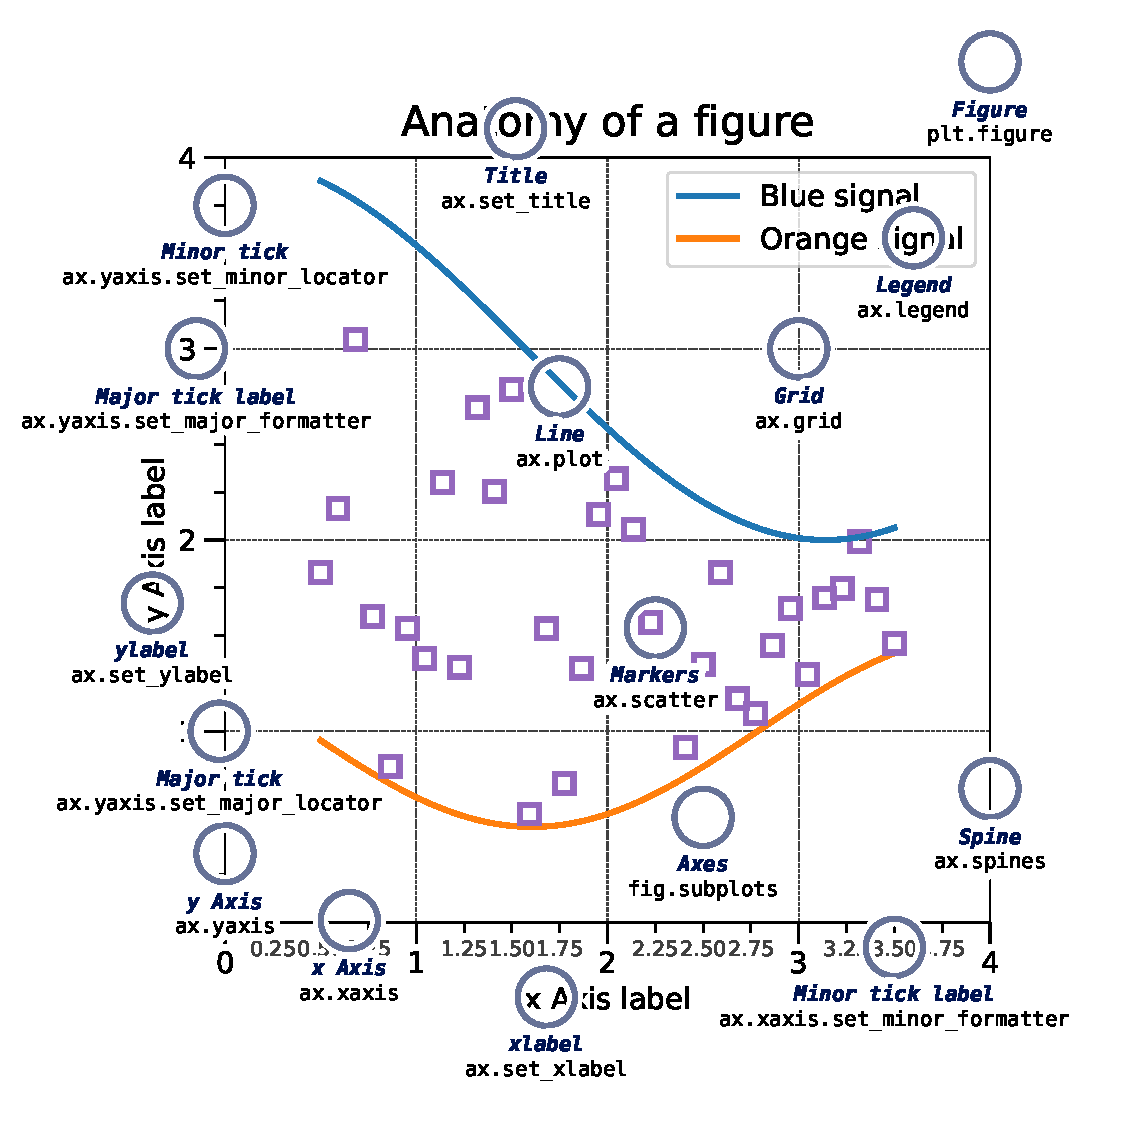
\includegraphics[width=0.8\linewidth]{capitulos/figuras/intro/figure_intro}
		\fonte{O autor.}
	\end{figure}
	
	A regra diz que a legenda fica sempre antes da figura, e a fonte após. Quando a figura for retirada de algum lugar, a fonte deve ser alterada para o padrão Autor, Ano. Ex.: Oliveira \textit{et al}, 2024
	
	


			
%% abtex2-modelo-include-comandos.tex, v-1.9.6 laurocesar
%% Copyright 2012-2016 by abnTeX2 group at http://www.abntex.net.br/ 
%%
%% This work may be distributed and/or modified under the
%% conditions of the LaTeX Project Public License, either version 1.3
%% of this license or (at your option) any later version.
%% The latest version of this license is in
%%   http://www.latex-project.org/lppl.txt
%% and version 1.3 or later is part of all distributions of LaTeX
%% version 2005/12/01 or later.
%%
%% This work has the LPPL maintenance status `maintained'.
%% 
%% The Current Maintainer of this work is the abnTeX2 team, led
%% by Lauro César Araujo. Further information are available on 
%% http://www.abntex.net.br/
%%
%% This work consists of the files abntex2-modelo-include-comandos.tex
%% and abntex2-modelo-img-marca.pdf
%%

% ---
% Este capítulo, utilizado por diferentes exemplos do abnTeX2, ilustra o uso de
% comandos do abnTeX2 e de LaTeX.
% ---

\chapter{Objetivos}
\label{objetivos}

	\section{Objetivos gerais}
	
		\lipsum[1-1]
		
	\section{Objetivos específicos}
	
		\lipsum[2-3]
	
		
%% abtex2-modelo-include-comandos.tex, v-1.9.6 laurocesar
%% Copyright 2012-2016 by abnTeX2 group at http://www.abntex.net.br/ 
%%
%% This work may be distributed and/or modified under the
%% conditions of the LaTeX Project Public License, either version 1.3
%% of this license or (at your option) any later version.
%% The latest version of this license is in
%%   http://www.latex-project.org/lppl.txt
%% and version 1.3 or later is part of all distributions of LaTeX
%% version 2005/12/01 or later.
%%
%% This work has the LPPL maintenance status `maintained'.
%% 
%% The Current Maintainer of this work is the abnTeX2 team, led
%% by Lauro César Araujo. Further information are available on 
%% http://www.abntex.net.br/
%%
%% This work consists of the files abntex2-modelo-include-comandos.tex
%% and abntex2-modelo-img-marca.pdf
%%

% ---
% Este capítulo, utilizado por diferentes exemplos do abnTeX2, ilustra o uso de
% comandos do abnTeX2 e de LaTeX.
% ---

\chapter{Metodologia}
\label{metodologia}

	\section{Exemplo de Seção}
	
		\lipsum[1-2]

		\subsection{Exemplo de Subseção}

			\lipsum[2-3]
		
		\subsection{Exemplo de Subseção}
		
			\lipsum[2-3]
			
			\subsubsection{Exemplo de Subsubseção}
			
				\lipsum[1-3]
	


%% abtex2-modelo-include-comandos.tex, v-1.9.6 laurocesar
%% Copyright 2012-2016 by abnTeX2 group at http://www.abntex.net.br/ 
%%
%% This work may be distributed and/or modified under the
%% conditions of the LaTeX Project Public License, either version 1.3
%% of this license or (at your option) any later version.
%% The latest version of this license is in
%%   http://www.latex-project.org/lppl.txt
%% and version 1.3 or later is part of all distributions of LaTeX
%% version 2005/12/01 or later.
%%
%% This work has the LPPL maintenance status `maintained'.
%% 
%% The Current Maintainer of this work is the abnTeX2 team, led
%% by Lauro César Araujo. Further information are available on 
%% http://www.abntex.net.br/
%%
%% This work consists of the files abntex2-modelo-include-comandos.tex
%% and abntex2-modelo-img-marca.pdf
%%

% ---
% Este capítulo, utilizado por diferentes exemplos do abnTeX2, ilustra o uso de
% comandos do abnTeX2 e de LaTeX.
% ---

\chapter{Conteúdos específicos do modelo de trabalho acadêmico}
\label{cap_trabalho_academico}

\section{Quadros}

Este modelo vem com o ambiente \texttt{quadro} e impressão de Lista de quadros configurados por padrão. Verifique um exemplo de utilização:

\begin{quadro}[htb]
	\caption{\label{quadro_exemplo}Exemplo de quadro}
	\begin{tabular}{|c|c|c|c|}
		\hline
		\textbf{Pessoa} & \textbf{Idade} & \textbf{Peso} & \textbf{Altura} \\ \hline
		Marcos & 26    & 68   & 178    \\ \hline
		Ivone  & 22    & 57   & 162    \\ \hline
		...    & ...   & ...  & ...    \\ \hline
		Sueli  & 40    & 65   & 153    \\ \hline
	\end{tabular}
	\fonte{Autor.}
\end{quadro}

Este parágrafo apresenta como referenciar o quadro no texto, requisito obrigatório da ABNT. Primeira opção, utilizando \texttt{autoref}: Ver o \autoref{quadro_exemplo}. Segunda opção, utilizando  \texttt{ref}: Ver o Quadro \ref{quadro_exemplo}.

\section{Código}

É possível também inserir blocos de código que se comportam como uma figura, como o exemplo apresentado na \autoref{MSER}.

\begin{figure}[!ht]
	\centering
	\caption{Exemplo de código para utilização do pyMSER. A função \texttt{equilibrate()} aplica o método MSER nos dados obtidos da simulação e gera um pequeno relatório com os resultados.}
	\label{MSER}
	\begin{lstlisting}[language=Python]
		import pymser
		import pandas as pd
		
		# Load the .csv file
		df = pd.read_csv('example_data/Cu-BTT_500165.0_198.000000.csv')
		
		results = pymser.equilibrate(
		df['mol/kg'], 
		LLM=True, 
		batch_size=1, 
		ADF_test=True, 
		uncertainty='uSD', 
		print_results=True
		)
	\end{lstlisting}
	\fonte{O autor.}
	
\end{figure}


\section{Tabela}

Em geral o modelo padrão de tabela do LaTeX pode ser meio feio, a \autoref{methods} apresenta um exemplo de tabela customizada. O comando \texttt{arraystretch} pode ser alterado para ajudar a redimensionar a tabela caso os dados sejam muito grandes para a folha. 

\begin{table}[ht!]
	\caption{Comparação entre tempo de execução, ponto de truncamento e valores médios da quantidade adsorvida obtidos com os diferentes métodos de equilibração no mesmo conjunto de dados.}
	\label{methods}
	\centering
	\renewcommand{\arraystretch}{1}
	\begin{tabular}{l|c|c|c}
		\hline\hline
		\textbf{Método} & \textbf{Tempo de execução (s)} & \textbf{t\textsubscript{0}} ($\times$10\textsuperscript{7}) & \textbf{Quant. adsorvida (mol/kg)} \\ \hline
		Gowers          & 0,05   & 2,57 & 39,85 $\pm$ 0,56 \\
		pyMSER          & 0,16   & 2,63 & 39,80 $\pm$ 0,56 \\
		RCA             & 0,51   & 5,92 & 40,24 $\pm$ 0,24 \\
		pyMBAR          & 78,93  & 7,69 & 40,07 $\pm$ 0,14 \\
		\hline \hline
	\end{tabular}
\end{table}


% ----------------------------------------------------------
% Finaliza a parte no bookmark do PDF
% para que se inicie o bookmark na raiz
% e adiciona espaço de parte no Sumário
% ----------------------------------------------------------
\phantompart

%% abtex2-modelo-include-comandos.tex, v-1.9.6 laurocesar
%% Copyright 2012-2016 by abnTeX2 group at http://www.abntex.net.br/ 
%%
%% This work may be distributed and/or modified under the
%% conditions of the LaTeX Project Public License, either version 1.3
%% of this license or (at your option) any later version.
%% The latest version of this license is in
%%   http://www.latex-project.org/lppl.txt
%% and version 1.3 or later is part of all distributions of LaTeX
%% version 2005/12/01 or later.
%%
%% This work has the LPPL maintenance status `maintained'.
%% 
%% The Current Maintainer of this work is the abnTeX2 team, led
%% by Lauro César Araujo. Further information are available on 
%% http://www.abntex.net.br/
%%
%% This work consists of the files abntex2-modelo-include-comandos.tex
%% and abntex2-modelo-img-marca.pdf
%%

% ---
% Este capítulo, utilizado por diferentes exemplos do abnTeX2, ilustra o uso de
% comandos do abnTeX2 e de LaTeX.
% ---

\chapter{Conclusão}
\label{conclusao}

	\lipsum[31-33]




% ----------------------------------------------------------
% ELEMENTOS PÓS-TEXTUAIS
% ----------------------------------------------------------
\postextual
% ----------------------------------------------------------

% ----------------------------------------------------------
% Referências bibliográficas
% ----------------------------------------------------------
\bibliography{referencias}

% ----------------------------------------------------------
% Glossário
% ----------------------------------------------------------
%
% Consulte o manual da classe abntex2 para orientações sobre o glossário.
%
%\glossary

% ----------------------------------------------------------
% Apêndices
% ----------------------------------------------------------

% ---
% Inicia os apêndices
% ---
\begin{apendicesenv}

% Imprime uma página indicando o início dos apêndices
\partapendices

%% abtex2-modelo-include-comandos.tex, v-1.9.6 laurocesar
%% Copyright 2012-2016 by abnTeX2 group at http://www.abntex.net.br/ 
%%
%% This work may be distributed and/or modified under the
%% conditions of the LaTeX Project Public License, either version 1.3
%% of this license or (at your option) any later version.
%% The latest version of this license is in
%%   http://www.latex-project.org/lppl.txt
%% and version 1.3 or later is part of all distributions of LaTeX
%% version 2005/12/01 or later.
%%
%% This work has the LPPL maintenance status `maintained'.
%% 
%% The Current Maintainer of this work is the abnTeX2 team, led
%% by Lauro César Araujo. Further information are available on 
%% http://www.abntex.net.br/
%%
%% This work consists of the files abntex2-modelo-include-comandos.tex
%% and abntex2-modelo-img-marca.pdf
%%

% ---
% Este capítulo, utilizado por diferentes exemplos do abnTeX2, ilustra o uso de
% comandos do abnTeX2 e de LaTeX.
% ---

% ----------------------------------------------------------
\chapter{Quisque libero justo}
% ----------------------------------------------------------

\lipsum[50]

% ----------------------------------------------------------
\chapter{Nullam elementum urna vel imperdiet sodales elit ipsum pharetra ligula
	ac pretium ante justo a nulla curabitur tristique arcu eu metus}
% ----------------------------------------------------------
\lipsum[55-57]



\end{apendicesenv}
% ---


% ----------------------------------------------------------
% Anexos
% ----------------------------------------------------------

% ---
% Inicia os anexos
% ---
\begin{anexosenv}

% Imprime uma página indicando o início dos anexos
\partanexos

%% abtex2-modelo-include-comandos.tex, v-1.9.6 laurocesar
%% Copyright 2012-2016 by abnTeX2 group at http://www.abntex.net.br/ 
%%
%% This work may be distributed and/or modified under the
%% conditions of the LaTeX Project Public License, either version 1.3
%% of this license or (at your option) any later version.
%% The latest version of this license is in
%%   http://www.latex-project.org/lppl.txt
%% and version 1.3 or later is part of all distributions of LaTeX
%% version 2005/12/01 or later.
%%
%% This work has the LPPL maintenance status `maintained'.
%% 
%% The Current Maintainer of this work is the abnTeX2 team, led
%% by Lauro César Araujo. Further information are available on 
%% http://www.abntex.net.br/
%%
%% This work consists of the files abntex2-modelo-include-comandos.tex
%% and abntex2-modelo-img-marca.pdf
%%

% ---
% Este capítulo, utilizado por diferentes exemplos do abnTeX2, ilustra o uso de
% comandos do abnTeX2 e de LaTeX.
% ---

\chapter{Morbi ultrices rutrum lorem.}
% ---
\lipsum[30]

% ---
\chapter{Cras non urna sed feugiat cum sociis natoque penatibus et magnis dis
	parturient montes nascetur ridiculus mus}
% ---

\lipsum[31]

% ---
\chapter{Fusce facilisis lacinia dui}
% ---

\lipsum[32]


\end{anexosenv}

%---------------------------------------------------------------------
% INDICE REMISSIVO
%---------------------------------------------------------------------
\phantompart
\printindex
%---------------------------------------------------------------------

\end{document}
